\chapter{Results and Discussion}\label{chap:results_discussion}

Within the scope of this thesis, our primary emphasis was on binary classification models. Although we did investigate regression models, the primary insights we obtained were predominantly derived from the analysis and evaluation of classification models. We have chosen not to include the results of the regression evaluation in this chapter because we recognized that the pivotal contributions are already achieved in the realm of classification.

\section{Binary Classification}
\subsection{Evaluation Metrics}
When assessing the performance of a binary prediction model using a validation dataset containing known target values, four key metrics come into play:

\begin{itemize}
  \item True Positives (TP): The number of correctly predicted active cases.
  \item True Negatives (TN): The number of correctly predicted inactive cases.
  \item False Positives (FP): The number of incorrectly predicted active cases.
  \item False Negatives (FN): The number of incorrectly predicted inactive cases.
\end{itemize}

With these four values, a confusion matrix can be created, as shown in Table~\ref{tab:confusion_matrix}.

\begin{table}[h]
  \centering
  \caption{Confusion Matrix}
  \label{tab:confusion_matrix}
  \setlength{\tabcolsep}{10pt} % Adjust cell padding
  \renewcommand{\arraystretch}{1.5} % Adjust cell height
  \begin{tabular}{|c|c|c|}
  \cline{2-3}
  \multicolumn{1}{c|}{} & Actual Negative & Actual Positive \\
  \hline
  Predicted Negative & TN & FN \\
  \hline
  Predicted Positive & FP & TP \\
  \hline
  \end{tabular}
\end{table}

In binary classification, the classification threshold is a crucial parameter dictating how the model assigns data points to one of two classes based on predicted class probabilities. This threshold significantly influences the model's metrics, as illustrated in Figure~\ref{fig:classification_threshold} and exemplified in Figure~\ref{fig:roc1120} and Figure~\ref{fig:cm1120}.
\begin{figure} 
  \centering
  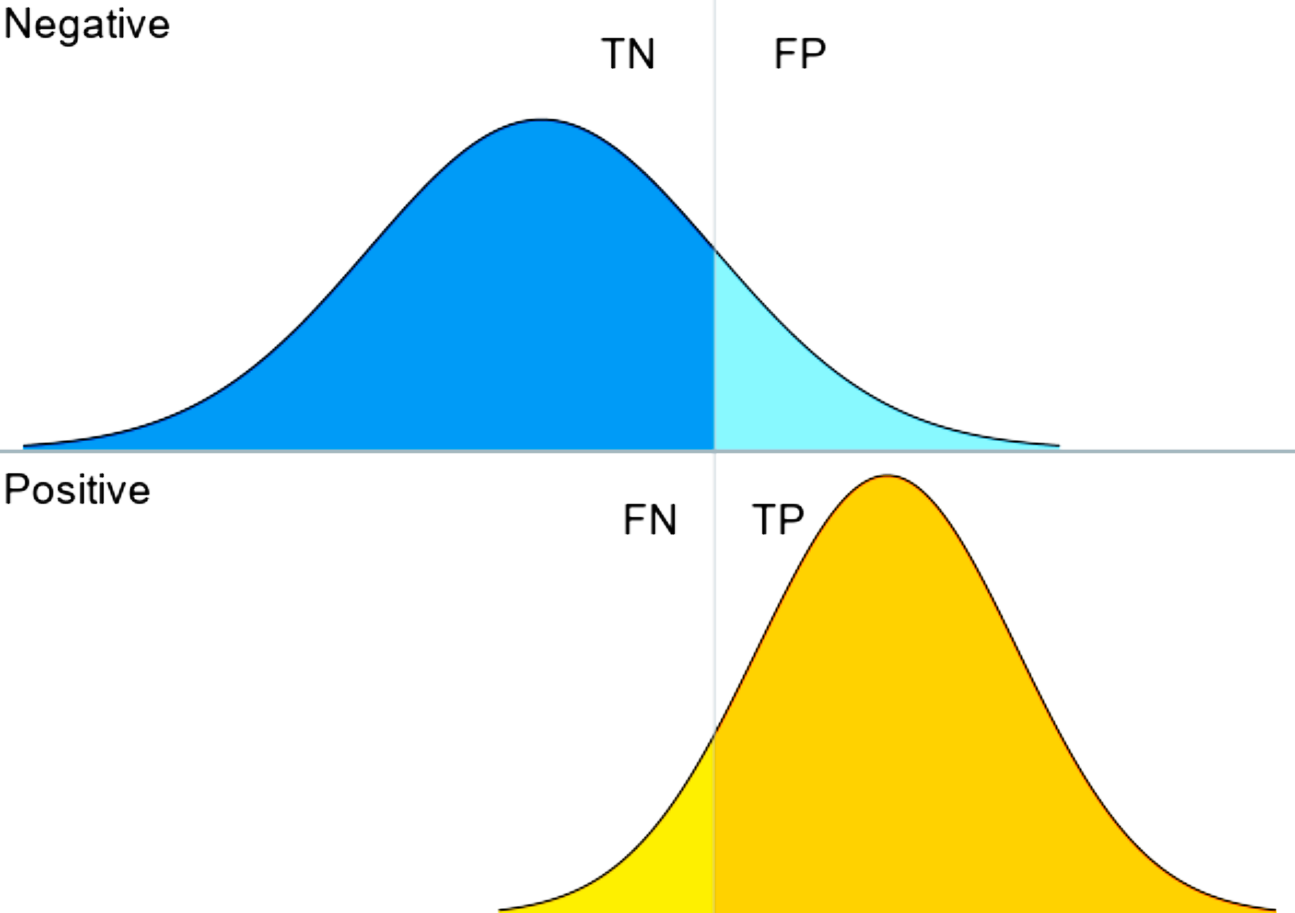
\includegraphics[width=0.5\textwidth]{figures/classification_threshold.png}
  \caption{Relationship between threshold and classification. Figure obtained from~\cite{wicklin2020}}
~\label{fig:classification_threshold}
\end{figure}

Various metrics assess predictive model performance, such as:

\begin{itemize}
  \item \textbf{Accuracy}: The ratio of correctly classified instances (TP) and (TN) to the total number of instances. It provides a general measure of the model's correctness.
  \[ \text{Accuracy}  A = \frac{TP + TN}{TP + TN + FP + FN} \]

  \item \textbf{Precision (P)}: The proportion of correctly predicted active cases (TP) to all instances predicted as active (TP + FP). 
  \[ \text{Precision } P = \frac{TP}{TP + FP} \]

  \item \textbf{Recall (R) or Sensitivity or True Positive Rate (TPR)}: The proportion of correctly predicted active cases (TP) to all actual active cases (TP + FN).
  \[ \text{Recall } R = \frac{TP}{TP + FN} \]

  \item \textbf{F1 Score}: The harmonic mean of precision and recall, which balances the trade-off between false positives and false negatives.
  \[ F1 = \frac{2 \cdot P \cdot R}{P + R} \]

  \item \textbf{True Negative Rate (TNR) Specificity}: The proportion of correctly predicted inactive cases (TN) to all actual inactive cases (TN + FP).
  \[ TNR = \frac{TN}{TN + FP} \]

  \item \textbf{Receiver Operating Characteristic (ROC) Curve}: A graphical representation of the model's performance across different classification thresholds. It plots the true positive rate (TNR) against the false positive rate (FPR), as exmplified for assay endpoint with aeid: 1120 in Figure~\ref{fig:roc1120}.
\end{itemize}

\begin{figure}[h]
  \centering
  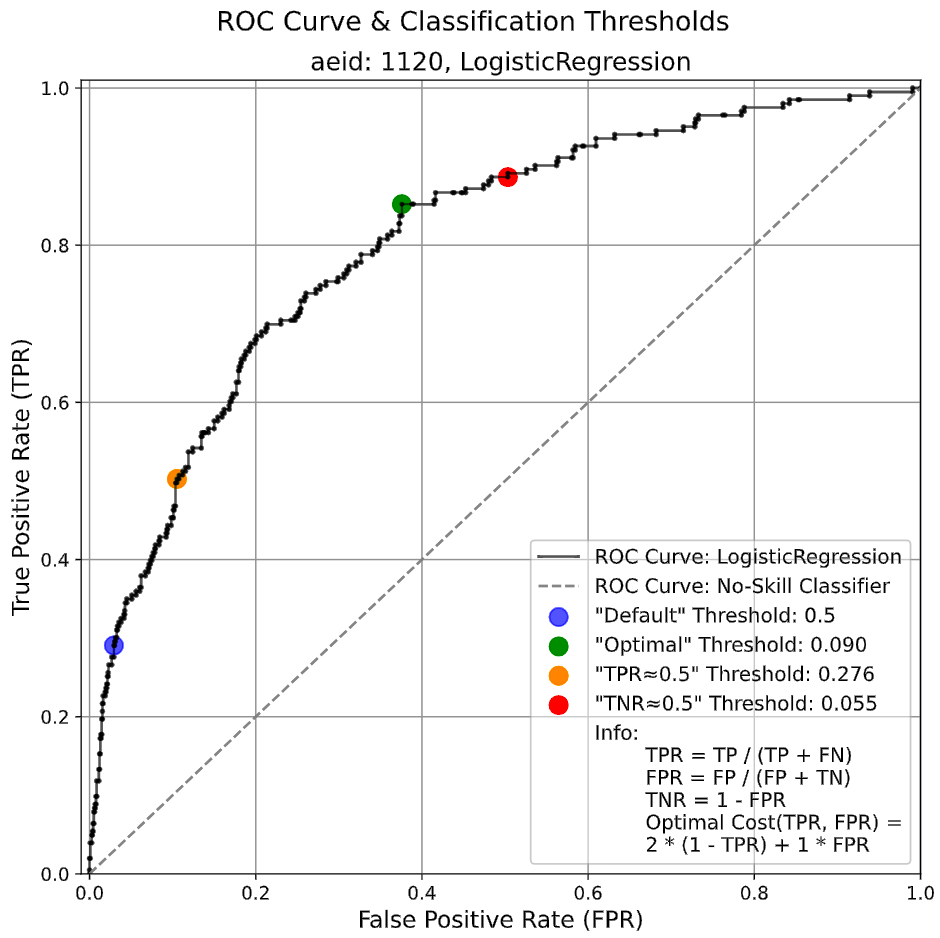
\includegraphics[width=0.7\textwidth]{figures/roc1120.png}
  \caption{The Receiver Operating Characteristic (ROC) curve is presented for the LogisticRegression classifier in the case of assay endpoint with aeid: 1120. We make predictions for each model combination using four distinct classification thresholds, specifically: the default threshold of 0.5, the optimal threshold determined by the cost function weighting TPR twice as FPR (to value recall), TPR approximately equal to 0.5, and TNR approximately equal to 0.5. Figure~\ref{fig:cm1120} shows the confusion matrices for the four thresholds.}
~\label{fig:roc1120}
\end{figure}

\begin{figure}[h]
  \centering
  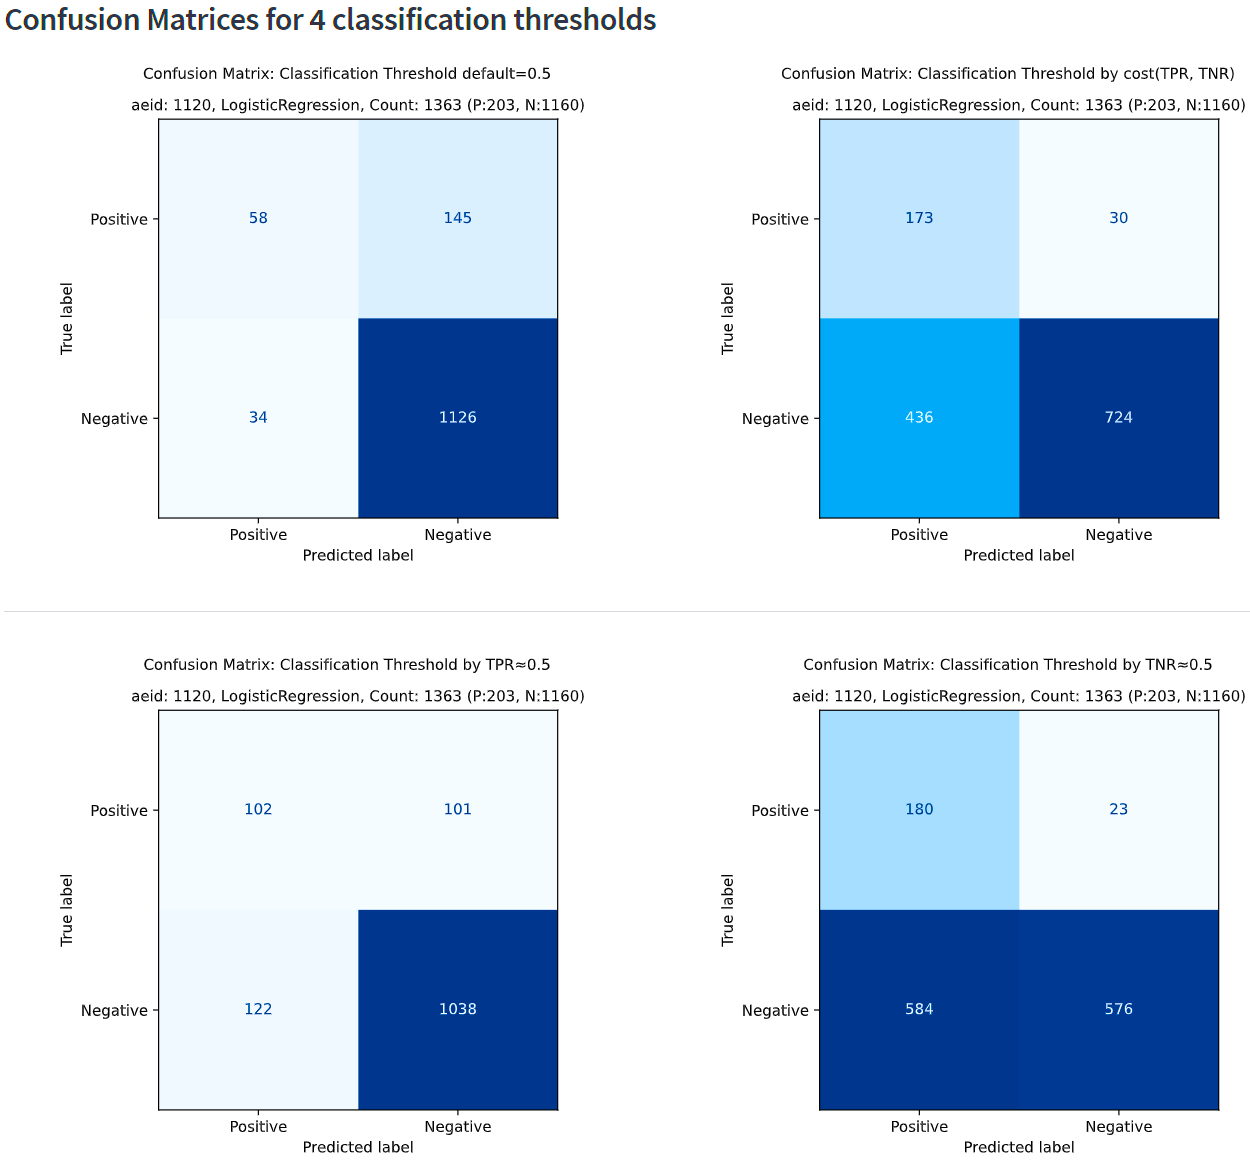
\includegraphics[width=1.0\textwidth]{figures/cm1120.png}
  \caption{For assay endpoint with aeid: 1120, confusion matrices are shown for four different classification thresholds.}
~\label{fig:cm1120}
\end{figure}

\subsubsection{Imbalanced Data}
A substantial proportion of the studied assay endpoints have an unequal distribution of active (positive) and inactive (negative) compounds. Typically, the negative class significantly outweights the positive class, as depicted by an example in Figure~\ref{fig:cm1120}. Such imbalanced datasets can result in skewed performance metrics, where the model may exhibit strong performance on the majority class while performing poorly on the minority class. To address imbalanced datasets, additional metrics such as macro averaged and weighted averaged metrics can be taken into account.
In macro averaging, the metric is computed separately for each class, and then an unweighted average is taken. This approach assigns equal importance to each class, regardless of their representation within the dataset. As an example, macro averaged precision calculates the unweighted average of precision across all classes, whereas the weighted average of precision considers the impact of class prevalence.
\[ \text{Macro Precision } = \frac{1}{N} \sum_{i=1}^{N} P_i \] 
\[ \text{Weighted Precision } = \frac{1}{N} \sum_{i=1}^{N} \left(\frac{TP_i}{TP_i + FP_i}\right) \cdot \frac{N_i}{N} \]

In both cases, $N$ is the total number of classes (e.g. $N=2$ for the binary case), and $N_i$ represents the number of samples in class $i$. Similarly the macro-averaged and weighted-averaged recall and F1 score can be calculated.


\subsection{Performance}

Performance results were generated for every combination of:

\begin{itemize}
  \item Target variables:
  \begin{enumerate}
    \item hitcall without cytotoxicity correction
    \item hitcall with cytotoxicity correction
  \end{enumerate}
  \item Assay endpoints ($\geq 300$):
  \item Feature selection models:
    \begin{enumerate}
      \item XGBoost
      \item RandomForest
    \end{enumerate}
    \item Estimator models:
    \begin{enumerate}
      \item LogisticRegression
      \item MLPClassifier
      \item RandomForestClassifier
      \item SVM (Support Vector Machine)
      \item XGBoostClassifier
    \end{enumerate}
  \item Validation sets:
    \begin{enumerate}
      \item the internal validation dataset 
      \item MassBank validation set with fingerprints from chemical structure
      \item MassBank validation set with SIRIUS-predicted fingerprints
    \end{enumerate}
  \item Classification thresholds:
    \begin{enumerate}
      \item $default$  (classification threshold of 0.5)
      \item $optimal$ (cost function weighting TPR twice as FPR)
      \item $TPR \simeq 0.5$ (TPR approximately equal to 0.5)
      \item $TNR \simeq 0.5$ (TNR approximately equal to 0.5)
    \end{enumerate}
  \item Metrics on:
    \begin{enumerate}
      \item macro average
      \item weighted average
      \item positive class
      \item negative class
    \end{enumerate}
\end{itemize}


Below, we provide figures illustrating the performance of binary classification models under the following configurations:
\begin{itemize}
  \item binarized hitcall without cytotoxicity correction
  \item XGBoost as the feature selection model
  \item the default classification threshold
\end{itemize}

With these fixed settings, we assessed the performance across all assay endpoints, estimator models, validation sets, and metrics. The figures are presented in the subsequent order:

\begin{table}[h]
  \centering
  \caption{Figure References and Descriptions}
  \begin{tabular}{lll}
    \toprule
    \textbf{Validation set} & \textbf{Metric} & \textbf{Figure} \\
    \midrule
    Internal & Macro averaged & Figure~\ref{fig:hitcall_classification_xgb_val_default_macro_avg} \\
    MassBank (from structure) & Macro averaged & Figure~\ref{fig:hitcall_classification_xgb_mb_val_structure_default_macro_avg} \\
    MassBank (SIRIUS-predicted) & Macro averaged & Figure~\ref{fig:hitcall_classification_xgb_mb_val_sirius_default_macro_avg} \\
    Internal & Weighted averaged & Figure~\ref{fig:hitcall_classification_xgb_val_default_weighted_avg} \\
    MassBank (from structure) & Weighted averaged & Figure~\ref{fig:hitcall_classification_xgb_mb_val_structure_default_weighted_avg} \\
    MassBank (SIRIUS-predicted) & Weighted averaged & Figure~\ref{fig:hitcall_classification_xgb_mb_val_sirius_default_weighted_avg} \\
    Internal  & Positve class & Figure~\ref{fig:hitcall_classification_xgb_val_default_true} \\
    MassBank (from structure)  & Positve class & Figure~\ref{fig:hitcall_classification_xgb_mb_val_structure_default_true} \\
    MassBank (SIRIUS-predicted)  & Positve class & Figure~\ref{fig:hitcall_classification_xgb_mb_val_sirius_default_true} \\
    Internal  & Negative class & Figure~\ref{fig:hitcall_classification_xgb_val_default_false} \\
    MassBank (from structure)  & Negative class & Figure~\ref{fig:hitcall_classification_xgb_mb_val_structure_default_false} \\
    MassBank (SIRIUS-predicted)  & Negative class & Figure~\ref{fig:hitcall_classification_xgb_mb_val_sirius_default_false} \\
    \bottomrule
  \end{tabular}
\end{table}

\begin{figure}
  \centering
  \includegraphics[width=0.99\textwidth]{figures/hitcall_classification_xgb_val_default_macro_avg.png}
  \caption{Internal validation set, macro averaged metrics. The marker size reflects the varying number of compounds in the validation set across the assay endpoints. The marginal boxplots illustrate the distribution of the performance metrics across the target assay endpoint models. The adjacent table provides the average metrics for the estimators across all target assay endpoint models.}
~\label{fig:hitcall_classification_xgb_val_default_macro_avg}
\end{figure}

\begin{figure}
  \centering
  \includegraphics[width=0.99\textwidth]{figures/hitcall_classification_xgb_mb_val_structure_default_macro_avg.png}
  \caption{MassBank validation set with fingerprints from chemical structure, macro averaged metrics.}
~\label{fig:hitcall_classification_xgb_mb_val_structure_default_macro_avg}
\end{figure}

\begin{figure}
  \centering
  \includegraphics[width=0.99\textwidth]{figures/hitcall_classification_xgb_mb_val_sirius_default_macro_avg.png}
  \caption{MassBank validation set with SIRIUS-predicted fingerprints, macro averaged metrics.}
~\label{fig:hitcall_classification_xgb_mb_val_sirius_default_macro_avg}
\end{figure}

\begin{figure}
  \centering
  \includegraphics[width=0.99\textwidth]{figures/hitcall_classification_xgb_val_default_weighted_avg.png}
  \caption{Internal validation set, weighted averaged metrics.}
~\label{fig:hitcall_classification_xgb_val_default_weighted_avg}
\end{figure}

\begin{figure}
  \centering
  \includegraphics[width=0.99\textwidth]{figures/hitcall_classification_xgb_mb_val_structure_default_weighted_avg.png}
  \caption{MassBank validation set with fingerprints from chemical structure, weighted averaged metrics.}
~\label{fig:hitcall_classification_xgb_mb_val_structure_default_weighted_avg}
\end{figure}

\begin{figure}
  \centering
  \includegraphics[width=0.99\textwidth]{figures/hitcall_classification_xgb_mb_val_sirius_default_weighted_avg.png}
  \caption{MassBank validation set with SIRIUS-predicted fingerprints, weighted averaged metrics.}
~\label{fig:hitcall_classification_xgb_mb_val_sirius_default_weighted_avg}
\end{figure}


\begin{figure}
  \centering
  \includegraphics[width=0.99\textwidth]{figures/hitcall_classification_xgb_val_default_true.png}
  \caption{Internal validation set, positive class metrics.}
~\label{fig:hitcall_classification_xgb_val_default_true}
\end{figure}

\begin{figure}
  \centering
  \includegraphics[width=0.99\textwidth]{figures/hitcall_classification_xgb_mb_val_structure_default_true.png}
  \caption{MassBank validation set with fingerprints from chemical structure, positive class metrics.}
~\label{fig:hitcall_classification_xgb_mb_val_structure_default_true}
\end{figure}

\begin{figure}
  \centering
  \includegraphics[width=0.99\textwidth]{figures/hitcall_classification_xgb_mb_val_sirius_default_true.png}
  \caption{MassBank validation set with SIRIUS-predicted fingerprints, positive class metrics.}
~\label{fig:hitcall_classification_xgb_mb_val_sirius_default_true}
\end{figure}


\begin{figure}
  \centering
  \includegraphics[width=0.99\textwidth]{figures/hitcall_classification_xgb_val_default_false.png}
  \caption{Internal validation set, negative class metrics.}
~\label{fig:hitcall_classification_xgb_val_default_false}
\end{figure}

\begin{figure}
  \centering
  \includegraphics[width=0.99\textwidth]{figures/hitcall_classification_xgb_mb_val_structure_default_false.png}
  \caption{MassBank validation set with fingerprints from chemical structure, negative class metrics.}
~\label{fig:hitcall_classification_xgb_mb_val_structure_default_false}
\end{figure}

\begin{figure}
  \centering
  \includegraphics[width=0.99\textwidth]{figures/hitcall_classification_xgb_mb_val_sirius_default_false.png}
  \caption{MassBank validation set with SIRIUS-predicted fingerprints, negative class metrics.}
~\label{fig:hitcall_classification_xgb_mb_val_sirius_default_false}
\end{figure}

\newpage
% \subsection{Feature Importance}

\section{Discussion}












